\chapter{Literature Review}
\label{LIT}
Many types of research and projects have already addressed the problem of generating sound and music through a textual representation instead of physical instruments. Many projects also consider the learning aspect of programming sound. This section provides on one site, how the in this thesis applied concepts are represented in the literature and on the other site, how related works cover the thesis' question. The related projects are ordered by relevance to this thesis, from less to more relevant. For each project, the basic concept is evaluated and discussed.

\section{Domain Specific Languages}
\label{LIT_DSL}
DSLs are not a new technology, in 1978 Ross described the Automatically-Programmed-Tools (APT) language, which was introduced for the United States Air Force in 1959.\cite{Ross1978} Ross conceived this language as a syntax for programming machine tools and performing operations on them. Fowler explains the growing interest in DSLs in the recent years by comparing the old programming language Lisp with the modern language Ruby on Rails.\cite{Fowler2010} He believes that the library and framework approach was influenced by the old programming language Lisp. Modern libraries and frameworks are similar to fluent interfaces and therefore to internal DSLs. Today, there are many of popular and important DSLs. But in some cases, these DSLs are not regarded as such. In addition to the technical introduction in \ref{THEO_DSL}, table \ref{TBL_DSLS} identifies multiple DSLs and their characteristic (internal or external) to support Fowler's statement that fluent interfaces play a substantial role.

\begin{table}[]
\caption{Popular DSL Examples and Types.}
\label{TBL_DSLS}
\begin{tabular}{p{150pt}|p{200pt}}
\rowcolor{htwg-teal} 
\textbf{DSL}                  			& \textbf{Type}     \\
SQL                  						& external \\
CSS                 						& external \\
Ant                  							& external \\
RegEx                						& external \\
Java's StringBuilder 				& internal \\
API's in general						& internal
\end{tabular}
\end{table}


The SQL \textit{language} is a good example of a fluent language. The listing \ref{LS_SQL} illustrates the query to get all products and their prices with the name \texttt{Coffee}. Once extracted and optional words are added, the query result is plain English.

\begin{lstlisting}[caption={SQL Fluent Language Example.}, label=LS_SQL]
SELECT ProductName, ProductPrice
FROM Product
WHERE ProductName = 'Coffee';
\end{lstlisting}

Fowler and Riti identify this readability as a "communication medium" with the domain experts: the "business people".\cite{Fowler2010, Riti2018} They explained that it is nowadays unavoidable that non-developers understand the purpose of a language-syntax.

Martin Fowler's "Domain-specific languages"\cite{Fowler2010} provides a well-founded theoretical groundwork of DSLs. It explains the theory behind DSLs in detail, without the impact of specific programming languages. Pierluigi Riti in "Practical Scala DSLs"\cite{Riti2018} offers real-world examples for the use of DSLs—internal and external. Riti implemented all examples in Scala. The work "DSLs in Action"\cite{Ghosh2010} from Debasish Ghosh is equivalent to Riti's, but with more theoretical background. Ghosh, however, uses different languages for his programming examples. "When and how to develop domain-specific languages"\cite{Mernik2005} from Marjan Mernik et al. discusses fundamental concepts of how to design a DSL and provides different patterns and implementation structures.

\section{Teaching Programming}
\label{LIT_TEACH}
"Computational Thinking", is a term Wing defined in 2006 as one key competency in children's education.\cite{Wing2006} She defines this therm detached from the assumption that children could have a carrier in computer science and places this skill alongside reading, writing and arithmetic. Wing's Computational Thinking emphasises the ability to analyse problems, categorise them and find a way to solve them.

Serafini refers to Wing's statement and is convinced that learning programming "on an adequate level of abstraction" supports this analytical ability.\cite{Serafini2011} Furthermore, Serafini does not limit Computational Thinking to children and extends it to all age groups. Serafini uses the programming language Logo to teach in primary schools. Logo is a "child-engineered version of Lisp"\cite{Kahn1995}, extended through graphics, which was developed in the '70s and is described in Serafini's research from 2011 as one of the most appropriate languages for novices.

Kahn developed 1995 ToomTalkTM, because of his critical view of the Logo language. Kahn follows another strategy and chooses animations to teach programming in his language. Because of Kahn's graphical approach, it is not covered in this thesis.\cite{Kahn1995}

Kranch's research provides a comprehensive study about teaching novice programmers.\cite{Kranch2012} He discusses questions like the starting point to teach programming and discusses the thinking process of novices and experts. He uses languages for teaching programming, which have their origin in fluent interfaces.

\section{Related Projects}
\label{LIT_PROJ}
This section presents related projects to this research in the order of their relevance. Close attention is paid to projects, which combine teaching programming and generating sound and music.

\subsection{SuperCollider}
\label{LIT_PROJ_SUPERCOLL}
\textit{SuperCollider}\footnote{SuperCollider - \url{https://supercollider.github.io}} is a development environment for realtime-audio-synthesis and algorithmic composition; it is a multi-platform tool and under the General Public License (GNU). SuperCollider contains two major components: \texttt{scsynth}, the real-time audio server and a dedicated interpreted programming language - \texttt{sclang}.\cite{SuperCollider}

The massive amount of disk space (the program reserves more than 240 MB in the unzipped version) and the synthesis approach make this an impractical option in cases where an \textit{easy to apply} music-layer is necessary. Although SuperCollider is a powerful tool to generate sounds on the base of audio-synthesis, it results in an unacceptable abstraction. Furthermore, the sclang language is questionable; listing \ref{LS_SUPER_FOREST} illustrates that sclang does not provide a fluent language.

\begin{lstlisting}[caption={SuperCollider's \texttt{sclang} Example: Forest Sound\cite{McCartney2007}}, label=LS_SUPER_FOREST]
{({
      RHPF.ar(
          OnePole.ar(BrownNoise.ar, 0.99),
          LPF.ar(BrownNoise.ar, 14) * 400 + 500, 0.03, 0.003
   )}!2)
   + 
   ({
      RHPF.ar(
          OnePole.ar(BrownNoise.ar, 0.99),
          LPF.ar(BrownNoise.ar, 20) * 800 + 1000, 0.03, 0.005
   )}!2)
}.play
\end{lstlisting}

\subsection{LilyPond}
\label{LIT_PROJ_LILY}
\textit{LilyPond}\footnote{LilyPond - \url{http://lilypond.org}} is a result of the lack of musicians and developers: Create digital sheet notes by hand in excellent quality to provide an approximation of traditional engraved music. The concept is to transform written notes (text) to sheet notes (images). It is also possible to generate a MIDI file from the written text.\cite{LilypoPage}

LilyPond is the state-of-the-art approach to write music. However, this project does not offer a fluent language, and the musician domain is preferred. Listing \ref{LS_LILY} and picture \ref{IMG_LILY} illustrate the transformation from the LilyPond language to sheet music. Although the notes and keywords are simple to understand and to read, the parentheses, square brackets, pointed brackets and backslashes are too intrusive.

\begin{lstlisting}[caption={Simple LilyPond Example - Input\cite{LilypoExmpl}}, label=LS_LILY]
\relative c' ' {
	\key c \minor
	g(
	<ees c'>)
	<d f gis b>-.
	<ees g bes>-.
}
\end{lstlisting}

\begin{figure}[h]
\caption{Simple LilyPond Example - Result\cite{LilypoExmpl}}
\label{IMG_LILY}
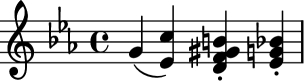
\includegraphics[scale=2]{lily}
\end{figure}

\subsection{Sonic Pi}
\label{LIT_PROJ_SONICPI}
An alternative approach was developed by Sam Aaron to connect the music and computer science subject in elementary schools. He developed and designed Sonic Pi together with teachers and students to the benefits from both sides—the novices and the educators.\cite{Blackwell2013, Aaron2016Art} In his article, Aaron describes his system "that may be easily understood by and taught to a ten-year-old child".\cite{Aaron2016Art} In 2013, he released Sonic Pi in version v1.0 and demonstrated together with the live coding environment Overtone the cardinality of DSLs and functional languages as a linguistic approach to teach music notation.\cite{Aaron2013}

The core advantage of Sonic Pi is timing. Version v1.0 presented a simple timing concept, which "resulted in badly timed music".\cite{Aaron2014} In 2014, Aaron introduced Sonic Pi in version v2.0 and presented a new time concept. The new concept of the real-time and "virtual-time" provides accurate timing which opened up Sonic Pi to a "Live Coding" environment.\cite{Aaron2014}

Through using the realtime-audio-synthesis system SuperCollider (cf. section \ref{LIT_PROJ_SUPERCOLL}) as "sound engine", Sonic Pi provides high quality sound synthesis which offers the opportunity for algorithmic music composition.

Listing \ref{LS_SONICPI-SEQ} illustrates the central approach to generate sequencing audio through Sonic Pi. The numbers \texttt{70}, \texttt{75} and \texttt{82} are MIDI-number representations. The sleep command is equivalent to the ordinary \texttt{thread sleep} construct; time is given in seconds.

\begin{lstlisting}[caption={Sonic Pi Sequencing Model\cite{Aaron2016Art}}, label=LS_SONICPI-SEQ]
play 70
sleep 1
play 75
sleep 1
play 82
\end{lstlisting}

Although, the Sonic Pi language adopts a fluent language in its most straightforward implementation. To enable more complex sound, the syntax is beyond this simplicity, as illustrated in listings \ref{LS_SONICPI_CONCUR} and \ref{LS_SONICPI_WOB}. Aaron adopted this approach to teach programming skills like multi-threading and functional programming due to the importance of these programming features in modern programming.\cite{Aaron2014} Unfortunately, Sonic Pi is not available as a web application, nor is it available for mobile devices; since it was initially developed for the RaspberryPi. There remains a need for a simple approach which combines the cardinality of Sonic Pi with a fluent language and the simplicity of a web-based application.

\begin{lstlisting}[caption={Sonic Pi Example - Concurrency\cite{Aaron2014}}, label=LS_SONICPI_CONCUR]
in_thread loop do play 30 sleep 0.5
end end
in_thread loop do sample :drum_heavy_kick sleep 1
end end
\end{lstlisting}
	
\begin{lstlisting}[caption={Sonic Pi Example - Wobling Sound\cite{SonicPi}}, label=LS_SONICPI_WOB]
with_fx :wobble, phase: 2 do |w|
  with_fx :echo, mix: 0.6 do
    loop do
      sample :drum_heavy_kick
      sample :bass_hit_c, rate: 0.8, amp: 0.4
      sleep 1
    end
  end
end
\end{lstlisting}


\subsection{ScalaKata2}
\label{LIT_PROJ_SCALAKATA2}
\textit{ScalaKata2}\footnote{ScalaKata2 - \url{https://github.com/MasseGuillaume/ScalaKata2}} is an interactive online playground for Scala. Developer Guillaume Massé implemented in 2016 an intuitive web-editor for compiling and executing Scala code. It offers syntax highlighting, code completion and error reporting, multi-room channels through WebSockets and code sharing to GitHub Gists. The editor CodeMirror, which is written in JavaScript, is used for the front-end development. ScalaKata2 communicates on the back-end side directly with the Scala compiler to compile and execute the written code and get the results. The project offers a convenient way to write code in a browser. The written code is sent to the corresponding server where it is evaluated and sent back to the front-end. Since these are already implemented features, ScalaKata2 provides a well-suited foundation for this thesis. The project is explained in more detail in chapter \ref{IMPL_SCALALAKATA}.

\subsection{Scalala}
\label{LIT_PROJ_SCALALA}
\textit{Scalala}\footnote{Scalala - \url{https://github.com/markoboger/scalala}}, developed by Marko Boger, offers an internal DSL written in Scala to play MIDI sound from REPL, Scala Worksheets or Scala code. It is implemented on the basis of the "Javax Midi class" which offers a way to play sounds directly with the related sound-board without generating an external MIDI file (c.f. section \ref{THEO_MIDI}). Furthermore, Boger used the Scala Actors API to implement the audio time management. The project provides already generic classes to map simple music elements to MIDI elements. The \texttt{key} and \texttt{instrument} class, for example, represent all available MIDI numbers to named-music-elements like \texttt{sharp}, \texttt{flat}, \texttt{piano}, \texttt{guitar} etc. Because of this, Scalala is used as a additional foundation for this study. It is explained in more detail in chapter \ref{IMPL_SCALALA}. 













